% This file was created with tikzplotlib v0.10.1.
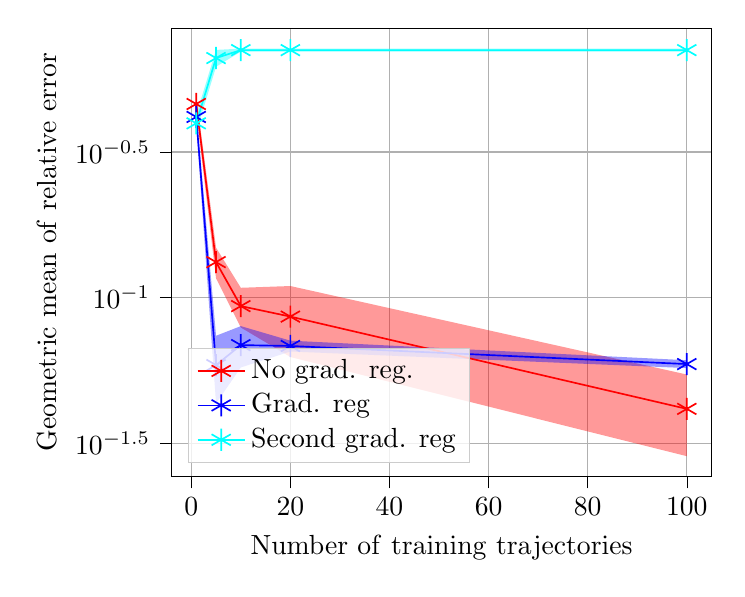
\begin{tikzpicture}

\definecolor{cyan}{RGB}{0,255,255}
\definecolor{darkgray176}{RGB}{176,176,176}
\definecolor{lightgray204}{RGB}{204,204,204}

\begin{axis}[
legend cell align={left},
legend style={
  fill opacity=0.8,
  draw opacity=1,
  text opacity=1,
  at={(0.03,0.03)},
  anchor=south west,
  draw=lightgray204
},
log basis y={10},
tick align=outside,
tick pos=left,
x grid style={darkgray176},
xlabel={\(\displaystyle \mathrm{Number \ of \ training \ trajectories }\)},
xmajorgrids,
xmin=-3.95, xmax=104.95,
xtick style={color=black},
y grid style={darkgray176},
ylabel={\(\displaystyle \mathrm{Geometric \ mean \ of \ relative \ error }\)},
ymajorgrids,
ymin=0.0243459387646996, ymax=0.840504356386208,
ymode=log,
ytick style={color=black}
]
\path [fill=red, fill opacity=0.4, semithick]
(axis cs:1,0.490901413014269)
--(axis cs:1,0.433024493967871)
--(axis cs:5,0.116525049895157)
--(axis cs:10,0.0790341389402467)
--(axis cs:20,0.0626124885872948)
--(axis cs:100,0.0285983365540995)
--(axis cs:100,0.0545071173413951)
--(axis cs:100,0.0545071173413951)
--(axis cs:20,0.109669975571805)
--(axis cs:10,0.108153574993502)
--(axis cs:5,0.148462798747811)
--(axis cs:1,0.490901413014269)
--cycle;

\path [fill=blue, fill opacity=0.4, semithick]
(axis cs:1,0.442382043258185)
--(axis cs:1,0.391624488446501)
--(axis cs:5,0.0433932534899063)
--(axis cs:10,0.0576485123326295)
--(axis cs:20,0.0653847632993373)
--(axis cs:100,0.0573638731354903)
--(axis cs:100,0.0610414733852138)
--(axis cs:100,0.0610414733852138)
--(axis cs:20,0.0712250882718893)
--(axis cs:10,0.0799055187974559)
--(axis cs:5,0.0740374694477401)
--(axis cs:1,0.442382043258185)
--cycle;

\path [fill=cyan, fill opacity=0.4, semithick]
(axis cs:1,0.423375587373515)
--(axis cs:1,0.369732728360975)
--(axis cs:5,0.619947094469653)
--(axis cs:10,0.698632973196945)
--(axis cs:20,0.698662782289567)
--(axis cs:100,0.698599796716216)
--(axis cs:100,0.715471014605402)
--(axis cs:100,0.715471014605402)
--(axis cs:20,0.715526497610524)
--(axis cs:10,0.715501788765345)
--(axis cs:5,0.708140271155905)
--(axis cs:1,0.423375587373515)
--cycle;

\addplot [semithick, red, mark=asterisk, mark size=4, mark options={solid}]
table {%
1 0.461962968111038
5 0.132493928074837
10 0.0935938507318497
20 0.0861412286758423
100 0.0415527261793613
};
\addlegendentry{No grad. reg.}
\addplot [semithick, blue, mark=asterisk, mark size=4, mark options={solid}]
table {%
1 0.417003273963928
5 0.0587153621017933
10 0.0687770172953606
20 0.0683049261569977
100 0.0592026822268963
};
\addlegendentry{Grad. reg}
\addplot [semithick, cyan, mark=asterisk, mark size=4, mark options={solid}]
table {%
1 0.39655414223671
5 0.664043605327606
10 0.707067430019379
20 0.707094609737396
100 0.707035422325134
};
\addlegendentry{Second grad. reg}
\end{axis}

\end{tikzpicture}
